\cleardoublepage
\chapter{STUDI LITERATUR}
\label{chap:studi-literatur}

\section{Diabetes Melitus Tipe 1 dan Pengelolaannya}
\label{sec:dmt1}

Diabetes melitus tipe 1 (DMT1) merupakan penyakit autoimun kronis yang ditandai oleh kerusakan sel beta pankreas, sehingga tubuh kehilangan kemampuan memproduksi insulin secara memadai \autocite{ada2026}. Kondisi ini berbeda secara mendasar dari diabetes tipe 2. Pada diabetes tipe 2 persoalan utamanya adalah resistensi terhadap insulin yang masih diproduksi tubuh, sedangkan pada DMT1 terjadi defisiensi insulin yang bersifat absolut \autocite{altobaishat2025}. Perbedaan mekanisme tersebut berimplikasi langsung pada tata laksananya. Penyandang DMT1 bergantung sepenuhnya pada insulin eksogen sepanjang hidup, sehingga penghentian terapi dalam waktu singkat dapat berakibat fatal.

Pengelolaan DMT1 pada praktiknya merupakan proses penyeimbangan yang berlangsung terus-menerus. Dosis insulin harus disesuaikan dengan asupan karbohidrat, tingkat aktivitas fisik, dan kondisi fisiologis lain yang berubah dari waktu ke waktu. Ketidakseimbangan ke satu arah menimbulkan hiperglikemia yang berkontribusi pada komplikasi jangka panjang, sedangkan ketidakseimbangan ke arah sebaliknya menimbulkan hipoglikemia yang berisiko akut dan dapat mengancam jiwa dalam hitungan menit. Asimetri risiko ini menjadi pertimbangan penting dalam merancang sistem pendukung keputusan, karena kesalahan prediksi ke arah bawah memiliki konsekuensi klinis yang lebih berat daripada kesalahan ke arah atas.

Standar penilaian pengendalian glukosa modern tidak lagi bertumpu hanya pada nilai rata-rata jangka panjang. Konsensus internasional memperkenalkan konsep \emph{time in range}, yaitu proporsi waktu ketika kadar glukosa berada dalam rentang sasaran, sebagai indikator yang lebih mencerminkan kualitas kendali glikemik harian \autocite{battelino2019}. Konsep tersebut menegaskan bahwa yang perlu dikelola bukan hanya tingkat glukosa rata-rata, melainkan juga stabilitasnya sepanjang hari. Perlu dicatat bahwa metrik tersebut didefinisikan di atas rekaman pemantauan kontinu dengan syarat kelengkapan data tertentu, sehingga tidak dapat dihitung dari catatan pemantauan mandiri yang bersifat periodik. Pada penelitian ini, konsep \emph{time in range} karena itu digunakan sebagai rujukan konseptual mengenai pentingnya stabilitas kadar glukosa, bukan sebagai metrik yang dihitung dari data penelitian.

Pada konteks Indonesia, pengelolaan DMT1 menghadapi tantangan tambahan. Rendahnya kesadaran masyarakat dan tenaga kesehatan menyebabkan sebagian besar pasien baru terdiagnosis setelah mengalami ketoasidosis diabetik \autocite{pulungan2021}. Ketersediaan tenaga ahli juga belum merata, sehingga rasio dokter endokrinologi anak terhadap jumlah pasien tergolong rendah dan pendampingan klinis berkelanjutan sulit diperoleh \autocite{faizi2025}.

\section{Pemantauan Glukosa dan Keterbatasannya}
\label{sec:pemantauan-glukosa}

Pemantauan kadar glukosa merupakan komponen inti pengelolaan DMT1 karena setiap keputusan terapi bergantung pada informasi tersebut. Terdapat dua pendekatan yang lazim digunakan. Pendekatan pertama adalah \emph{continuous glucose monitoring} (CGM), yaitu sensor yang merekam kadar glukosa secara otomatis dalam interval beberapa menit. Pendekatan kedua adalah pemantauan mandiri melalui pengukuran tusuk jari (\emph{finger-stick}) menggunakan glukometer, yang hasilnya dicatat secara manual dalam bentuk \emph{logbook}.

Perbedaan keduanya tidak berhenti pada tingkat kenyamanan maupun karakteristik data, melainkan mencakup besaran fisiologis yang diukur. CGM mengukur kadar glukosa pada cairan interstisial sebagai penaksir kadar glukosa plasma, sedangkan pengukuran tusuk jari mengukur kadar glukosa pada darah kapiler \autocite{holt2021}. Keduanya karena itu bukan besaran yang identik meskipun sama-sama dinyatakan dalam satuan yang sama. Perbedaan ini perlu dinyatakan sejak awal karena evaluasi pada Bab~\ref{chap:evaluasi} menggunakan pembacaan tusuk jari sebagai masukan dan kanal CGM sebagai nilai acuan, sehingga penyetaraan keduanya merupakan asumsi metodologis yang disadari dan bukan kesetaraan yang diandaikan begitu saja.

Selain perbedaan besaran tersebut, terdapat pula perbedaan pada karakteristik data yang dihasilkan. CGM menghasilkan deret waktu yang rapat dan teratur, sehingga memungkinkan analisis tren secara rinci. Sebaliknya, pencatatan \emph{logbook} menghasilkan data yang jarang, tidak teratur, dan bergantung pada kedisiplinan pencatatan. Sebagian besar penelitian prediksi glukosa mengasumsikan ketersediaan data bertipe pertama, sedangkan kenyataan di lapangan pada lingkungan dengan sumber daya terbatas lebih sering menyerupai tipe kedua.

Keterbatasan tersebut berakar pada persoalan keterjangkauan. Survei harga di Indonesia menunjukkan bahwa pengadaan glukometer beserta pasokan strip uji bulanan menimbulkan beban biaya yang signifikan bagi pekerja berpenghasilan rendah, sementara insulin turut menambah beban tersebut \autocite{ramadaniati2024}. Perangkat CGM yang harganya berlipat lebih mahal karena itu belum terjangkau oleh mayoritas pasien. Persoalan yang sama teramati di negara berkembang lain, sehingga kesenjangan akses teknologi DMT1 antara negara maju dan negara berkembang tetap lebar \autocite{santoscastro2025}. Di Indonesia, kondisi ini diperberat oleh cakupan jaminan kesehatan nasional yang belum menanggung perangkat pemantauan mandiri \autocite{faizi2025}.

Konsekuensi metodologisnya penting untuk penelitian ini. Sistem yang dirancang untuk lingkungan dengan sumber daya terbatas tidak dapat mengandalkan ketersediaan aliran data kontinu. Sistem tersebut harus mampu bekerja di atas data periodik yang jarang, dengan konsekuensi bahwa informasi tren jangka pendek perlu direkonstruksi melalui rekayasa fitur, bukan diperoleh langsung dari sensor.

\section{Faktor-Faktor yang Memengaruhi Kadar Glukosa}
\label{sec:faktor-glukosa}

Kadar glukosa darah dipengaruhi oleh interaksi sejumlah faktor yang bekerja pada skala waktu berbeda. Pemahaman atas faktor-faktor tersebut menjadi landasan pemilihan fitur pada model prediksi yang dibahas pada Bab~\ref{chap:perancangan}. Secara klasik, dinamika glukosa, insulin, dan karbohidrat dimodelkan melalui pendekatan fisiologis seperti \emph{minimal model} yang dirumuskan \textcite{bergman1979}, yang kemudian dikembangkan menjadi simulator fisiologis yang lebih lengkap \autocite{dallaman2014}. Penelitian ini tidak mengadopsi pemodelan fisiologis tersebut secara langsung, tetapi menggunakannya sebagai dasar konseptual untuk merancang fitur yang merepresentasikan efek residual insulin dan karbohidrat.

\subsection{Asupan Karbohidrat}
\label{subsec:karbohidrat}

Asupan karbohidrat memberikan dampak paling langsung terhadap kenaikan kadar glukosa setelah makan. Karbohidrat dihidrolisis menjadi glukosa dan diserap ke aliran darah dalam rentang waktu tertentu, sehingga efeknya tidak muncul seketika melainkan tersebar selama beberapa jam. Pada DMT1, ketiadaan insulin endogen menyebabkan kenaikan tersebut tidak dapat dikompensasi secara otomatis oleh tubuh, sehingga penyesuaian dosis insulin sepenuhnya bergantung pada perhitungan eksternal. Karena efeknya bersifat tertunda dan meluruh, penelitian ini merepresentasikan asupan karbohidrat melalui besaran \emph{carbohydrate on board} (COB), bukan melalui nilai mentah pada setiap catatan.

\subsection{Insulin}
\label{subsec:insulin}

Insulin menurunkan kadar glukosa dengan durasi kerja yang meluruh selama beberapa jam setelah pemberian. Akibatnya, dosis yang diberikan pada suatu waktu masih memberikan efek pada periode berikutnya.

Pemberian insulin pada terapi DMT1 terdiri atas dua komponen yang berbeda sifatnya. Pembedaan itulah yang menentukan cara keduanya direpresentasikan. Insulin \emph{basal} diberikan secara terus-menerus untuk memenuhi kebutuhan metabolisme dasar, sehingga nilainya hampir selalu ada pada setiap titik waktu. Insulin \emph{bolus} diberikan secara diskret pada waktu makan atau untuk koreksi hiperglikemia, sehingga bernilai nol pada sebagian besar titik waktu. Komponen yang menimbulkan persoalan representasi adalah bolus, karena justru komponen inilah yang bersifat sesaat namun berefek panjang. Penelitian ini karena itu merepresentasikan \emph{bolus} melalui besaran \emph{insulin on board} (IOB) dengan model peluruhan eksponensial, sedangkan basal yang bersifat kontinu tidak memerlukan representasi meluruh.

\subsection{Aktivitas Fisik}
\label{subsec:aktivitas-fisik}

Aktivitas fisik meningkatkan sensitivitas insulin dan pada umumnya menurunkan kadar glukosa, meskipun besaran serta arah efeknya dapat bervariasi menurut jenis dan intensitas aktivitas \autocite{colberg2016}. Faktor ini diperlakukan sebagai variabel sekunder yang relevan dalam prediksi.

\subsection{Faktor Psikologis}
\label{subsec:faktor-psikologis}

Stres psikologis memicu respons neuroendokrin yang meningkatkan kadar kortisol dan menurunkan efektivitas kerja insulin, sehingga berpotensi menaikkan kadar glukosa. Pengaruh tersebut telah diamati secara langsung pada penyandang DMT1. \textcite{velasco2022} memantau sepuluh pasien DMT1 menggunakan sensor glukosa sambil mengumpulkan laporan mandiri mengenai tingkat stres, lalu menemukan bahwa rerata glukosa pada kondisi tenang sebesar 126,56~mg/dL, lebih rendah secara bermakna dibandingkan 147,96~mg/dL pada kondisi normal dan 146,13~mg/dL pada kondisi gugup. Selain rerata, ukuran variabilitas berupa simpangan baku, koefisien variasi, dan amplitudo rata-rata ekskursi glikemik juga meningkat seiring naiknya tingkat stres. Temuan tersebut menunjukkan bahwa stres memengaruhi bukan hanya tinggi rendahnya kadar glukosa, melainkan juga kestabilannya.

Perlu dicatat bahwa penelitian tersebut melibatkan jumlah partisipan yang terbatas dan mengandalkan penilaian subjektif pasien, sebagaimana diakui penulisnya. Meskipun demikian, cara pengumpulan datanya sejalan dengan ketersediaan informasi stres pada dataset yang digunakan penelitian ini, yaitu berupa pelaporan mandiri. Faktor ini karena itu diperlakukan sebagai variabel pendukung yang digunakan apabila tersedia.

\subsection{Efek Residual Insulin dan Karbohidrat}
\label{subsec:efek-residual}

Ketiga faktor yang telah dibahas pada Subbab~\ref{subsec:karbohidrat} hingga Subbab~\ref{subsec:aktivitas-fisik} memiliki satu sifat bersama, yaitu pengaruhnya tidak berhenti pada saat kejadian berlangsung. Satu dosis insulin yang disuntikkan pada suatu waktu masih bekerja beberapa jam sesudahnya, sedangkan satu porsi karbohidrat yang dikonsumsi masih diserap setelah waktu makan berakhir. Akibatnya, kadar glukosa pada suatu waktu tidak hanya ditentukan oleh kejadian pada waktu tersebut, melainkan juga oleh sisa pengaruh kejadian sebelumnya.

Sifat tersebut menimbulkan persoalan pada perancangan fitur model prediksi. Fitur yang hanya mencatat dosis insulin atau asupan karbohidrat pada satu titik waktu akan bernilai nol pada seluruh titik waktu lainnya, sehingga model kehilangan informasi mengenai pengaruh yang masih berlangsung. Dua besaran yang lazim digunakan untuk mengatasi hal ini adalah \emph{insulin on board} (IOB) dan \emph{carbohydrate on board} (COB). Keduanya menyatakan jumlah insulin dan karbohidrat yang secara efektif masih aktif pada suatu waktu, dihitung dari akumulasi kejadian sebelumnya yang meluruh seiring berjalannya waktu.

Pemodelan fisiologis yang lengkap atas kedua proses tersebut memerlukan sistem persamaan berkompartemen banyak sebagaimana dirumuskan pada \emph{minimal model} \textcite{bergman1979} dan pengembangannya \autocite{dallaman2014}. Pemodelan penuh tersebut mensyaratkan parameter fisiologis per pasien yang tidak tersedia pada data \emph{logbook}. Penelitian ini karena itu menggunakan penyederhanaan berupa peluruhan eksponensial orde pertama, yaitu nilai IOB dan COB pada suatu waktu dihitung sebagai penjumlahan masukan baru dengan nilai sebelumnya yang telah diredam oleh faktor peluruhan. Penyederhanaan ini mempertahankan sifat pokok yang hendak direpresentasikan, yaitu pengaruh yang menurun secara bertahap dan bukan berhenti seketika, tanpa menuntut parameter yang tidak dapat diperoleh. Rumusan lengkap beserta nilai parameternya disajikan pada Bab~\ref{chap:perancangan}. Perbandingan antara kedua bentuk representasi tersebut ditunjukkan pada Gambar~\ref{fig:iob-cob}.

\begin{figure}[htbp]
\centering
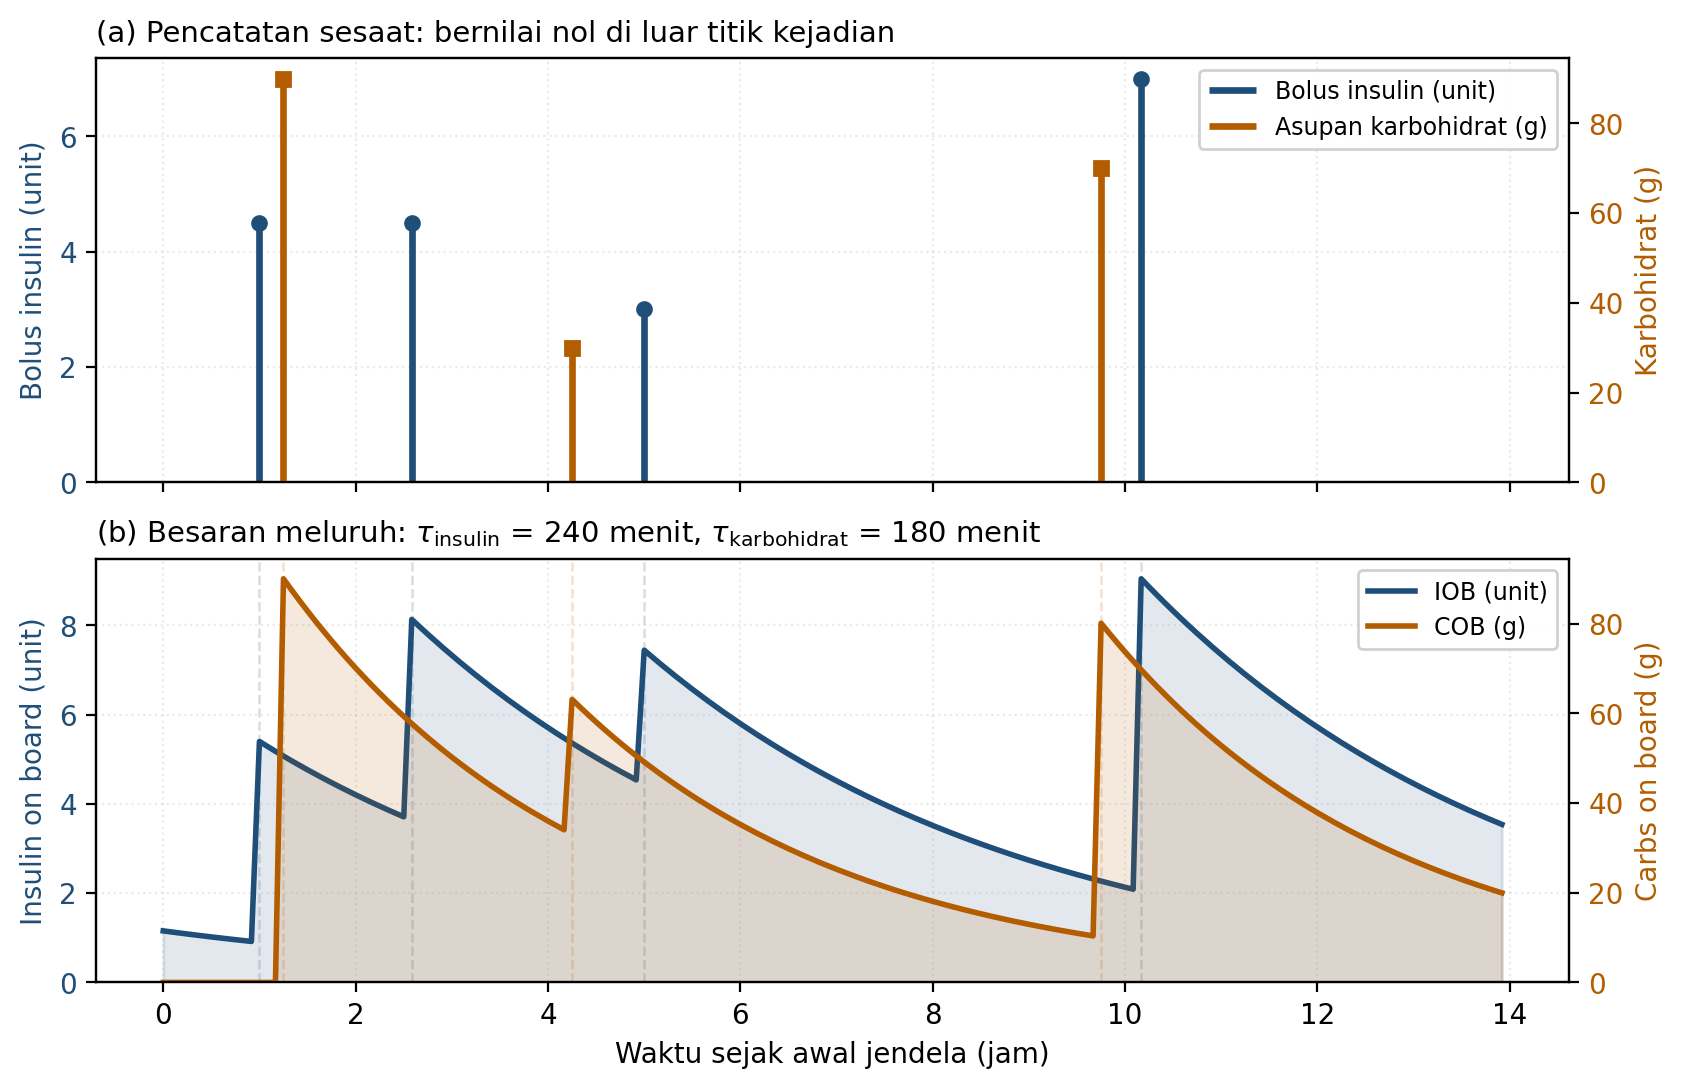
\includegraphics[width=\textwidth]{images/Gambar_II5_IOBCOB.png}
\caption{Perbandingan pencatatan kejadian sesaat dan besaran meluruh pada satu jendela 14 jam dari dataset OhioT1DM.}
\label{fig:iob-cob}
\end{figure}

Gambar~\ref{fig:iob-cob} memperlihatkan dua hal yang menjadi alasan pemilihan representasi ini. Pertama, panel (a) menunjukkan bahwa pemberian bolus dan asupan karbohidrat tercatat sebagai kejadian terpisah yang bernilai nol pada seluruh titik waktu di antaranya, sehingga model yang membacanya secara mentah tidak memperoleh informasi apa pun mengenai pengaruh yang masih berlangsung. Kedua, panel (b) menunjukkan bahwa besaran IOB dan COB tidak hanya meluruh, melainkan juga \emph{bertumpuk}: ketika kejadian baru muncul sebelum pengaruh kejadian sebelumnya habis, nilainya bertambah di atas sisa yang masih ada. Pada jendela tersebut, misalnya, bolus kedua menaikkan IOB dari sekitar 3,7 unit menjadi sekitar 8,1 unit karena bolus pertama masih menyisakan pengaruh. Sifat penumpukan inilah yang tidak dapat diwakili oleh pencatatan sesaat, padahal justru sifat itu yang menentukan besar risiko hipoglikemia.

Laju peluruhan pada perhitungan tersebut ditentukan oleh konstanta waktu yang mencerminkan lama kerja masing-masing zat. Untuk insulin, PERKENI mencantumkan bahwa insulin analog kerja cepat memiliki awitan 5 hingga 15 menit, puncak efek 1 hingga 2 jam, dan lama kerja 4 hingga 6 jam \autocite{perkeni2021insulin}. Rentang tersebut menjadi dasar penetapan konstanta waktu insulin pada penelitian ini. Untuk karbohidrat, tidak dijumpai rentang tunggal yang berlaku umum karena laju penyerapan bergantung pada komposisi makanan, kandungan serat, dan indeks glikemik \autocite{annan2022}. Konstanta waktu karbohidrat karena itu diperlakukan sebagai parameter rancangan yang ditetapkan secara empiris. Pengaruh pemilihan nilainya diuji pada Bab~\ref{chap:evaluasi}.

\section{Prediksi Kadar Glukosa Berbasis \emph{Machine Learning}}
\label{sec:prediksi-ml}

Pendekatan berbasis data memungkinkan prediksi fluktuasi glukosa dari riwayat pengukuran, sehingga risiko hipoglikemia maupun hiperglikemia dapat diantisipasi sebelum kejadiannya berlangsung \autocite{woldaregay2019}. Model dilatih atas pasangan masukan berupa kadar glukosa sebelumnya beserta variabel pendukung, serta keluaran berupa kadar glukosa pada waktu berikutnya. Dua kelas model yang relevan bagi penelitian ini adalah \emph{ensemble} berbasis pohon keputusan dan jaringan saraf rekuren.

\subsection{\emph{Ensemble} Berbasis Pohon Keputusan}
\label{subsec:ensemble-pohon}

Kedua model \emph{ensemble} yang digunakan pada penelitian ini, yaitu \emph{Random Forest} dan \emph{Gradient Boosting Machine}, sama-sama menggabungkan banyak pohon keputusan. Perbedaannya terletak pada \emph{cara} penggabungan itu dilakukan. Perbedaan itulah yang berkonsekuensi langsung pada ukuran model, ketersediaan taksiran ketidakpastian, serta keterbatasan yang sama-sama dimiliki keduanya.

\paragraph{\emph{Random Forest} sebagai \emph{bagging}.} \emph{Random Forest} melatih banyak pohon secara \emph{paralel} dan saling bebas, masing-masing atas sampel \emph{bootstrap} dan subset fitur yang dipilih acak, kemudian merata-ratakan prediksinya \autocite{breiman2001}. Mekanisme ini bekerja dengan menekan \emph{varians}: tiap pohon dibiarkan tumbuh dalam sehingga bias rendah tetapi varians tinggi, sedangkan perata-rataan atas banyak pohon meredam varians tersebut. Dua konsekuensi mengikuti. Pertama, model yang tersimpan memuat banyak pohon berkedalaman penuh, sehingga ukurannya besar. Kedua, karena pohon-pohon tersebut saling bebas, sebaran prediksi antarpohon dapat langsung ditafsirkan sebagai taksiran ketidakpastian per sampel tanpa mekanisme tambahan.

\paragraph{\emph{Gradient Boosting} sebagai \emph{boosting}.} \emph{Gradient Boosting Machine} melatih pohon secara \emph{berurutan}, dengan setiap pohon baru dilatih untuk mengoreksi galat sisa dari gabungan pohon sebelumnya, mengikuti arah gradien negatif fungsi kerugian \autocite{friedman2001}. Mekanisme ini bekerja dengan menekan \emph{bias}: tiap pohon dibiarkan dangkal sehingga secara sendirian lemah, tetapi rangkaian koreksi berurutan menghasilkan model yang kuat. Konsekuensinya berkebalikan dengan \emph{bagging}. Pertama, model yang tersimpan memuat banyak pohon dangkal, sehingga ukurannya jauh lebih ringkas. Kedua, karena pohon-pohon tersebut saling bergantung dan bukan penaksir yang berdiri sendiri, sebaran antarpohon tidak dapat ditafsirkan sebagai ketidakpastian, sehingga taksiran ketidakpastian per sampel harus diperoleh melalui mekanisme lain.

Implementasi \emph{gradient boosting} berbasis histogram membagi nilai fitur kontinu ke dalam sejumlah tetap \emph{bin} sebelum pencarian titik pisah dilakukan, sehingga biaya pencarian bergantung pada jumlah \emph{bin} dan bukan pada jumlah sampel \autocite{ke2017}. Sifat ini menjadikannya sepadan secara komputasi pada himpunan jendela berukuran ratusan ribu, sebagaimana yang dihadapi penelitian ini.

\paragraph{Keterbatasan yang dimiliki keduanya.} Kedua model tersebut, dalam bentuk regresi yang digunakan pada penelitian ini, sama-sama meminimalkan galat kuadrat. Fungsi kerugian tersebut memberi bobot yang sebanding dengan kuadrat selisih, sehingga penaksir optimalnya cenderung menyusut ke arah nilai tengah sebaran. Pada data glukosa, kejadian ekstrem berupa hipoglikemia merupakan kelas yang jarang, sehingga penyusutan tersebut membuat kedua model jarang menghasilkan nilai yang melewati ambang bawah. Keterbatasan ini karena itu melekat pada \emph{fungsi kerugian}, bukan pada keluarga model, dan konsekuensinya terhadap sensitivitas deteksi hipoglikemia dibahas pada Bab~\ref{chap:evaluasi}.

\subsection{\emph{Long Short-Term Memory}}
\label{subsec:lstm}

\emph{Long Short-Term Memory} (LSTM) merupakan varian \emph{recurrent neural network} yang mampu menangkap dependensi jangka panjang pada data deret waktu melalui \emph{memory cell} dan mekanisme gerbang, sehingga mengatasi persoalan \emph{vanishing gradient} pada RNN standar \autocite{hochreiter1997}. Arsitektur ini banyak dipakai pada prediksi kadar glukosa karena data pemantauan bersifat berurutan menurut waktu \autocite{woldaregay2019}. Meskipun demikian, kemampuan generalisasi model \emph{deep learning} antar-dataset masih menjadi tantangan yang terdokumentasi \autocite{ghimire2024}.

\subsection{Perbandingan Karakteristik Ketiga Model}
\label{subsec:perbandingan-model}

Ketiga model tersebut dievaluasi sebagai pembanding penuh pada Bab~\ref{chap:evaluasi}. Perbandingan karakteristiknya secara konseptual disajikan pada Tabel~\ref{tab:perbandingan-model}.

% =====================================================================
% BARIS TERAKHIR ("Kesesuaian dengan konteks penelitian") TERTAHAN.
%
% Dua alasan lama pemilihan Random Forest sudah DICABUT (KEPUTUSAN #5):
%   - keterjelasan kontribusi fitur : digugurkan J7. Yang dimiliki RF secara
%     bawaan adalah MDI, dan MDI tidak boleh dilaporkan karena bias
%     kardinalitas; angka yang dilaporkan adalah permutation importance
%     yang MODEL-AGNOSTIK sehingga bukan keunggulan RF.
%   - kebutuhan komputasi rendah    : terbalik secara faktual.
%
% Isi baris tersebut setelah keputusan Random Forest / Gradient Boosting
% ditetapkan. Rujukan: docs/ALUR_SISTEM_FINAL.md, docs/KEPUTUSAN_DIAMBIL.md
% =====================================================================
\begin{longtable}{@{}p{2.5cm}p{3.9cm}p{3.9cm}p{3.9cm}@{}}
\caption{Perbandingan karakteristik \emph{Random Forest}, \emph{Gradient Boosting Machine}, dan LSTM.}
\label{tab:perbandingan-model} \\
\toprule
\textbf{Aspek} & \textbf{Random Forest} & \textbf{Gradient Boosting} & \textbf{LSTM} \\
\midrule
\endfirsthead

\multicolumn{4}{@{}l}{\small\emph{Tabel \thetable{} (lanjutan)}} \\
\toprule
\textbf{Aspek} & \textbf{Random Forest} & \textbf{Gradient Boosting} & \textbf{LSTM} \\
\midrule
\endhead

\bottomrule
\endlastfoot

Mekanisme penggabungan & \emph{Bagging}: pohon dilatih paralel dan saling bebas, prediksinya dirata-ratakan untuk menekan varians & \emph{Boosting}: pohon dilatih berurutan, tiap pohon mengoreksi galat sisa pendahulunya untuk menekan bias & Pemrosesan berurutan melalui \emph{memory cell} dan mekanisme gerbang \\[2pt]

Kedalaman pohon & Dalam, agar bias tiap pohon rendah & Dangkal, karena kekuatan berasal dari rangkaian koreksi & Tidak berlaku \\[2pt]

Penanganan deret waktu & Ketergantungan temporal harus dinyatakan eksplisit melalui rekayasa fitur & Ketergantungan temporal harus dinyatakan eksplisit melalui rekayasa fitur & Ketergantungan temporal dimodelkan secara langsung \\[2pt]

Ketidakpastian per sampel & Tersedia bawaan dari sebaran prediksi antarpohon yang saling bebas & Tidak tersedia bawaan; pohon saling bergantung sehingga sebarannya tidak bermakna & Tidak tersedia bawaan \\[2pt]

Kebutuhan volume data & Dapat dilatih pada data berukuran sedang & Dapat dilatih pada data berukuran sedang & Umumnya menuntut volume data lebih besar untuk kinerja yang stabil \\[2pt]

Kebutuhan komputasi & Bergantung pada jumlah dan kedalaman pohon & Bergantung pada jumlah pohon dan jumlah \emph{bin} histogram & Bergantung pada ukuran jaringan dan panjang jendela masukan \\[2pt]

Generalisasi antar-dataset & Bergantung pada kesamaan sebaran fitur antara data latih dan uji & Bergantung pada kesamaan sebaran fitur antara data latih dan uji & Kinerja menurun pada data yang berbeda dari data pelatihan \\[2pt]

Keterbatasan bersama & \multicolumn{2}{p{7.9cm}}{Keduanya meminimalkan galat kuadrat, sehingga penaksirnya menyusut ke arah nilai tengah dan jarang melewati ambang pada kelas yang jarang muncul} & Bergantung pada fungsi kerugian yang dipilih \\[2pt]

Kesesuaian dengan konteks penelitian & Memenuhi batasan tanpa akselerator grafis, tetapi ukuran artefaknya besar sehingga membebani penyimpanan dan waktu muat & \textbf{Dipilih.} Memenuhi batasan tanpa akselerator grafis dengan artefak dan waktu pelatihan yang jauh lebih kecil, serta menyediakan jalur regresi dan jalur klasifikasi pada satu keluarga model & Menuntut akselerator grafis untuk pelatihan yang praktis, sehingga bertentangan dengan Batasan~4 \\

\end{longtable}

\noindent\footnotesize Disusun berdasarkan \textcite{breiman2001}, \textcite{friedman2001}, \textcite{ke2017}, \textcite{hochreiter1997}, dan \textcite{ghimire2024}. Baris kebutuhan komputasi dan baris ketidakpastian menyatakan sifat mekanisme, bukan hasil pengukuran; nilai terukur pada penelitian ini disajikan pada Bab~\ref{chap:evaluasi}.\normalsize


Tabel~\ref{tab:perbandingan-model} memperlihatkan bahwa tidak terdapat model yang unggul pada seluruh aspek. Keunggulan LSTM terletak pada kemampuannya memodelkan ketergantungan temporal secara langsung tanpa rekayasa fitur eksplisit. Keunggulan \emph{Gradient Boosting} terletak pada keringkasan model dan biaya pelatihan yang rendah sebagai akibat dari penggunaan pohon dangkal. Adapun \emph{Random Forest} menyediakan taksiran ketidakpastian per sampel secara bawaan melalui sebaran antarpohon. Perlu ditekankan bahwa baris kebutuhan komputasi dan baris ketidakpastian pada tabel tersebut menyatakan \emph{sifat mekanisme}, bukan hasil pengukuran; nilai terukur pada penelitian ini seluruhnya disajikan pada Bab~\ref{chap:evaluasi}.

\subsection{Horizon Prediksi dan Penilaian Keamanan Klinis}
\label{subsec:horizon-keamanan}

Horizon prediksi yang digunakan pada penelitian ini adalah 30 menit dan 60 menit ke depan. Penetapan tersebut bersandar pada dasar klinis berupa lingkar waktu tindakan, yang diuraikan pada Subbab~\ref{subsec:horizon-prediksi}, sekaligus pada konvensi yang lazim dipakai penelitian prediksi glukosa di atas dataset OhioT1DM \autocite{marling2020} sehingga hasilnya dapat diperbandingkan.

Penilaian kualitas prediksi tidak cukup dilakukan melalui metrik galat konvensional saja. Dua prediksi dengan besar galat yang sama dapat memiliki konsekuensi klinis yang sangat berbeda, bergantung pada arah kesalahan dan rentang kadar glukosa tempat kesalahan itu terjadi. Untuk itu digunakan \emph{Clarke Error Grid Analysis}, yang memetakan pasangan nilai aktual dan prediksi ke dalam zona A sampai E menurut konsekuensi klinis dari keputusan yang akan diambil berdasarkan prediksi tersebut \autocite{clarke1987}. Perinciannya dibahas pada Bab~\ref{chap:evaluasi}.

\subsection{Kuantifikasi Ketidakpastian Prediksi}
\label{subsec:ketidakpastian}

Keluaran modul prediksi sejauh ini dibahas sebagai nilai tunggal, yaitu satu angka taksiran kadar glukosa pada horizon tertentu. Bentuk keluaran tersebut menyembunyikan satu informasi yang bernilai klinis, yaitu seberapa yakin model terhadap taksirannya. Dua prediksi dengan nilai yang sama dapat memiliki tingkat keyakinan yang berbeda, misalnya ketika yang satu dihitung dari pola yang sering ditemui pada data pelatihan sedangkan yang lain dihitung dari kombinasi masukan yang jarang muncul. Klinisi yang menerima kedua prediksi tersebut dalam bentuk angka tunggal tidak memiliki dasar untuk membedakan keduanya.

Kebutuhan akan informasi ketidakpastian ini bertaut langsung dengan asimetri risiko yang telah diuraikan pada Subbab~\ref{sec:dmt1}. Ketika prediksi mengarah pada kadar glukosa yang mendekati batas bawah, konsekuensi dari kesalahan tidak setara ke kedua arah. Rentang taksiran yang menyertakan kemungkinan kadar glukosa turun lebih rendah daripada nilai titiknya memberikan dasar tindakan yang berbeda dibandingkan rentang taksiran yang seluruhnya berada di atas ambang aman, meskipun nilai titik keduanya identik. Dengan demikian, penyajian ketidakpastian bukan tambahan teknis, melainkan bagian dari penyampaian informasi yang aman secara klinis.

Salah satu kerangka yang dapat digunakan untuk keperluan tersebut adalah \emph{conformal prediction}. Kerangka ini menghasilkan interval prediksi dengan jaminan cakupan pada tingkat kepercayaan yang ditetapkan, tanpa mensyaratkan asumsi mengenai sebaran data maupun bentuk model yang digunakan \autocite{angelopoulos2021}. Prosedurnya bertumpu pada sehimpunan data kalibrasi yang terpisah dari data pelatihan. Besar galat model pada data kalibrasi digunakan untuk menetapkan lebar interval, sehingga interval yang dihasilkan mencerminkan perilaku galat yang teramati dan bukan asumsi teoretis.

Sifat kerangka ini yang tidak bergantung pada jenis model membuatnya dapat diterapkan pada ketiga model yang dibandingkan tanpa mengubah arsitekturnya. Meskipun demikian, penaksir ketidakpastian per sampel yang menjadi masukannya berbeda menurut keluarga model, sebagaimana diuraikan pada Subbab~\ref{subsec:ensemble-pohon}. Pada model \emph{bagging}, sebaran prediksi antarpohon dapat langsung digunakan. Pada model \emph{boosting}, penaksir tersebut harus diperoleh melalui mekanisme lain, misalnya melalui model kuantil yang dilatih terpisah. Perbedaan ini tidak memengaruhi jaminan cakupan yang dihasilkan, karena kuantil konformal yang dihitung pada himpunan kalibrasi menyerap skala penaksir apa pun yang digunakan.

Jaminan cakupan yang dihasilkan bersifat marginal, yaitu berlaku rata-rata atas keseluruhan data uji dan tidak dijamin berlaku seragam pada setiap subkelompok kondisi. Keterbatasan tersebut penting untuk dinyatakan karena rentang kadar glukosa yang paling kritis secara klinis justru merupakan rentang yang paling jarang muncul pada data. Penerapan kerangka ini pada penelitian ini beserta hasil pengukuran cakupannya dibahas pada Bab~\ref{chap:evaluasi}.

\section{Sistem Pendukung Keputusan Klinis}
\label{sec:cdss}

Sistem pendukung keputusan klinis (\emph{clinical decision support system}, CDSS) adalah sistem yang menyediakan informasi tersaring kepada tenaga kesehatan pada waktu yang tepat untuk mendukung pengambilan keputusan \autocite{sutton2020}. Sistem tersebut telah lama digunakan dalam berbagai bentuk, mulai dari pengingat sederhana hingga sistem berbasis pengetahuan yang kompleks. Manfaat yang dilaporkan mencakup peningkatan kepatuhan terhadap pedoman klinis dan pengurangan kesalahan, sementara risikonya mencakup kelelahan akibat peringatan yang berlebihan serta ketergantungan berlebih pada keluaran sistem.

Karakteristik penting CDSS adalah posisinya sebagai pendukung, bukan pengganti, penilaian klinis. Penelitian ini mengikuti prinsip tersebut melalui alur \emph{doctor-mediated}, yaitu rekomendasi yang dihasilkan sistem divalidasi terlebih dahulu oleh dokter sebelum sampai kepada pasien. Rancangan ini menempatkan tanggung jawab klinis tetap pada tenaga kesehatan, sekaligus mengurangi risiko yang timbul apabila keluaran sistem keliru.

Dalam kerangka CDSS, keadaan pasien perlu direpresentasikan dalam bentuk yang dapat diproses sistem. Penelitian ini merepresentasikannya sebagai vektor fitur ringkas yang dihitung dari catatan \emph{logbook}, mencakup kadar glukosa terakhir, besaran IOB dan COB, indikator tren, serta penanda waktu. Representasi ini bersifat ringkas dan diperbarui ketika data baru dimasukkan, tanpa melibatkan sinkronisasi otomatis dengan sensor.

\section{\emph{Retrieval-Augmented Generation}}
\label{sec:rag}

\subsection{Arsitektur dan Taksonomi}
\label{subsec:arsitektur-rag}

\emph{Retrieval-Augmented Generation} (RAG) memadukan pencarian dokumen dari basis pengetahuan eksternal dengan kemampuan generatif model bahasa besar \autocite{lewis2020}. Arsitekturnya terdiri atas dua komponen utama. Komponen pertama adalah \emph{retriever}, yang mengambil potongan dokumen relevan melalui pencarian berbasis vektor. Komponen kedua adalah \emph{generator}, yang menyusun keluaran berdasarkan konteks hasil pencarian tersebut. Dalam implementasinya, dokumen diubah menjadi representasi vektor menggunakan model \emph{embedding} seperti Sentence-BERT \autocite{reimers2019}, kemudian disimpan pada basis data vektor untuk memungkinkan pencarian semantik. Alur kerja kedua komponen tersebut ditunjukkan pada Gambar~\ref{fig:arsitektur-rag}.

\begin{figure}[htbp]
\centering
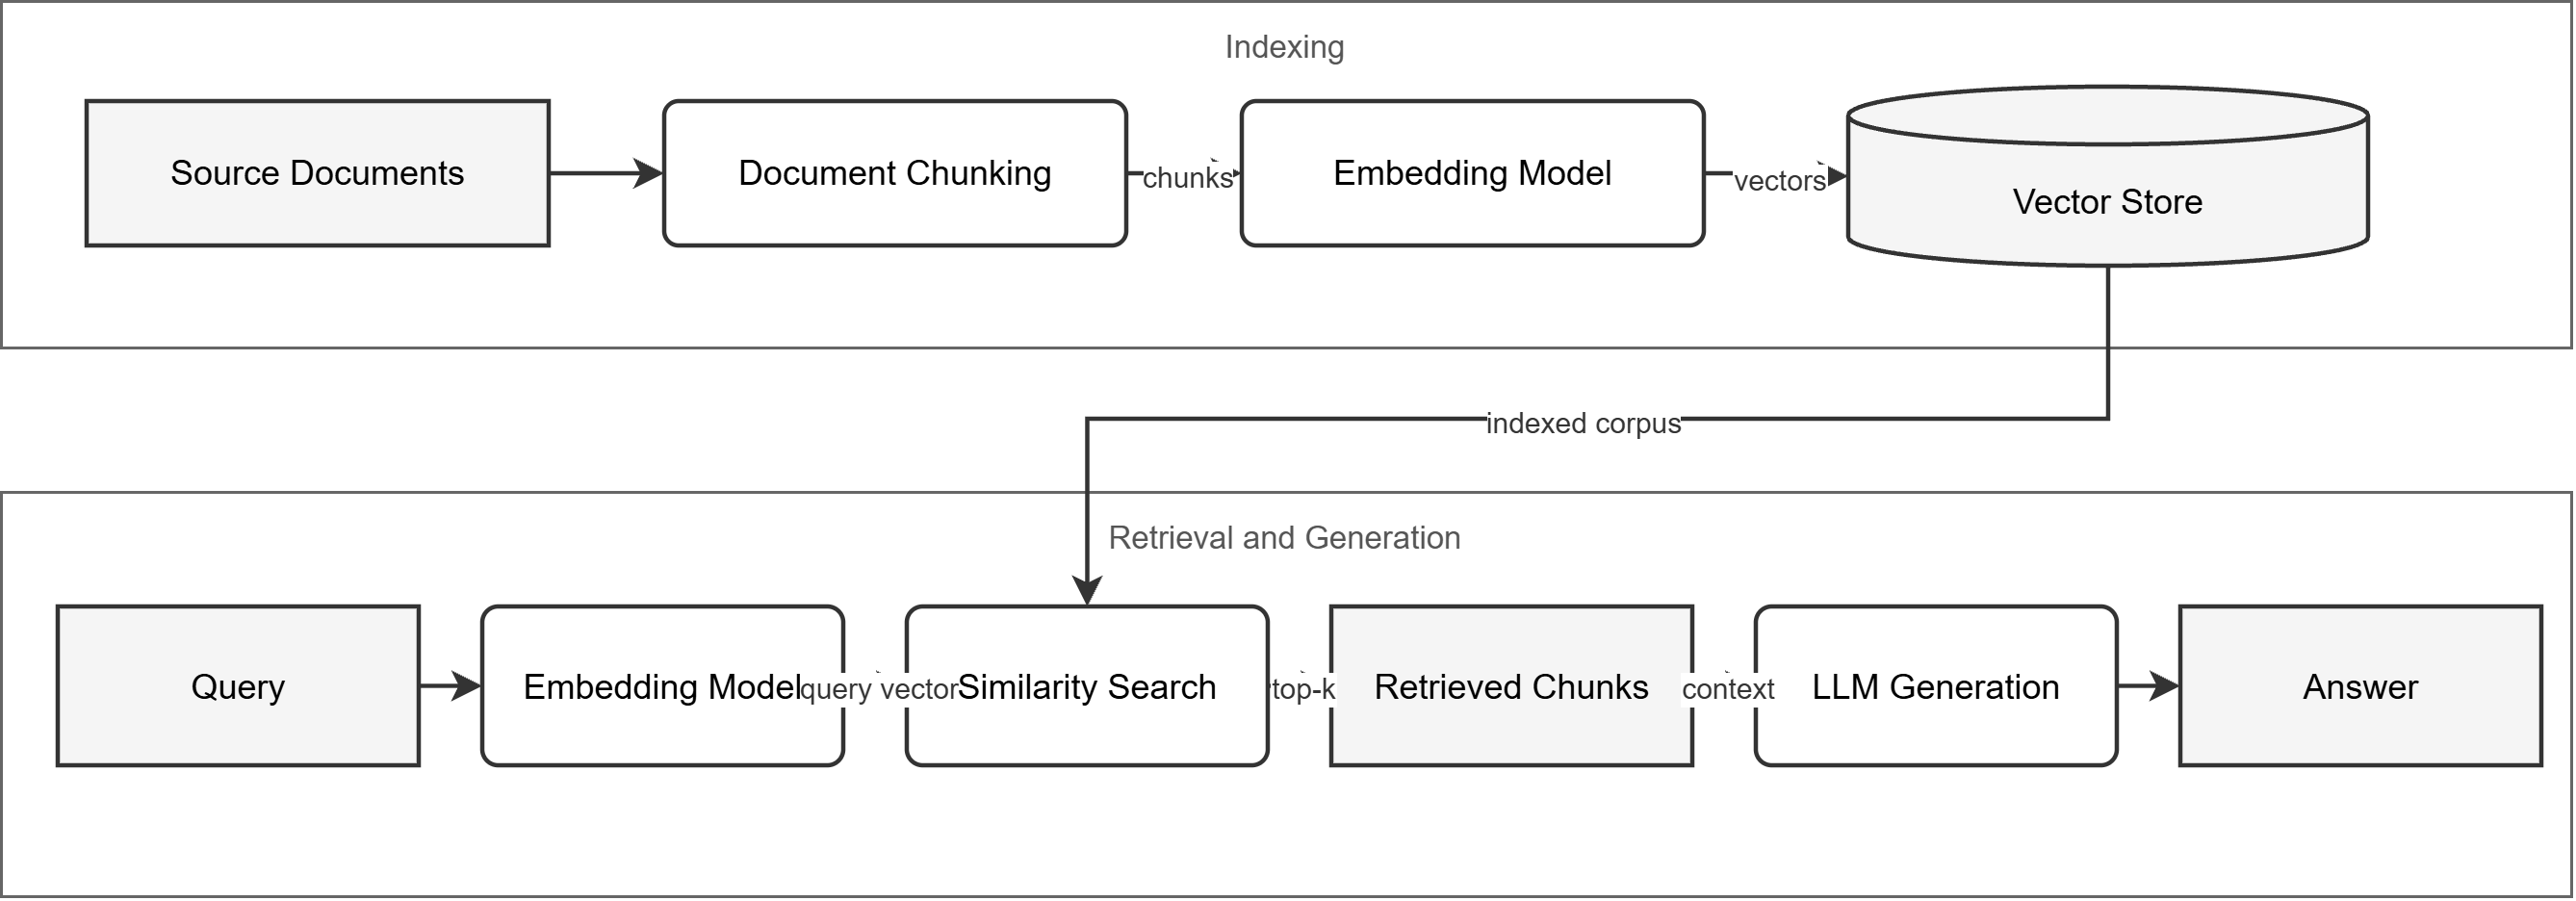
\includegraphics[width=\textwidth]{images/Gambar_II1_ArsitekturRAG.png}
\caption{Arsitektur RAG standar, mencakup tahap pengindeksan serta tahap penelusuran dan pembangkitan.}
\label{fig:arsitektur-rag}
\end{figure}

Gambar~\ref{fig:arsitektur-rag} memperlihatkan bahwa alur dimulai dari kueri yang diubah menjadi representasi vektor, dilanjutkan dengan pencarian pada basis data vektor, pengambilan potongan dokumen yang paling relevan, hingga pembangkitan jawaban oleh model bahasa dengan potongan dokumen tersebut sebagai konteks. Struktur inilah yang menjadi tulang punggung sistem pada penelitian ini. Keunggulan utama pendekatan ini terletak pada tiga hal. Pertama, pengetahuan dapat diperbarui dengan mengganti korpus dokumen tanpa melatih ulang model bahasa. Kedua, keluaran dapat ditelusuri sumbernya sehingga lebih mudah diverifikasi. Ketiga, risiko halusinasi dapat ditekan karena jawaban dibumikan pada dokumen yang benar-benar ada.

Satu sifat model \emph{embedding} yang perlu diperhatikan pada penelitian ini adalah keterbatasannya dalam menangani lebih dari satu bahasa. Model yang dilatih pada korpus satu bahasa memetakan kalimat berbahasa lain ke wilayah ruang vektor yang berbeda meskipun maknanya sama, sehingga pencarian lintas bahasa menjadi tidak dapat diandalkan. \textcite{reimers2020} mengatasi hal ini melalui distilasi pengetahuan, yaitu melatih model agar kalimat terjemahan dipetakan ke posisi yang sama dengan kalimat aslinya pada ruang vektor. Persoalan ini relevan karena korpus pedoman pada penelitian ini memuat dokumen berbahasa Indonesia dan berbahasa Inggris sekaligus, sementara kueri dan keluaran sistem menggunakan bahasa Indonesia. Konsekuensi pemilihan model \emph{embedding} terhadap kondisi tersebut dibahas pada Bab~\ref{chap:analisis-masalah}.

Perkembangan RAG kemudian melahirkan berbagai varian yang dirangkum \textcite{gao2023} ke dalam tiga paradigma, yaitu RAG standar, RAG canggih, dan RAG modular. RAG standar menjalankan alur tunggal berupa pengubahan kueri menjadi vektor, pencarian dokumen, lalu pembangkitan jawaban. RAG canggih menambahkan optimasi pada tahap sebelum atau sesudah pencarian, misalnya melalui transformasi kueri (\emph{query transformation}) atau pemeringkatan ulang hasil. RAG modular menyusun komponen-komponen tersebut secara lebih fleksibel, termasuk melalui iterasi dan penggunaan agen. Ketiga paradigma tersebut beserta letak penelitian ini di dalamnya dipetakan pada Gambar~\ref{fig:paradigma-rag}.

\begin{figure}[htbp]
\centering
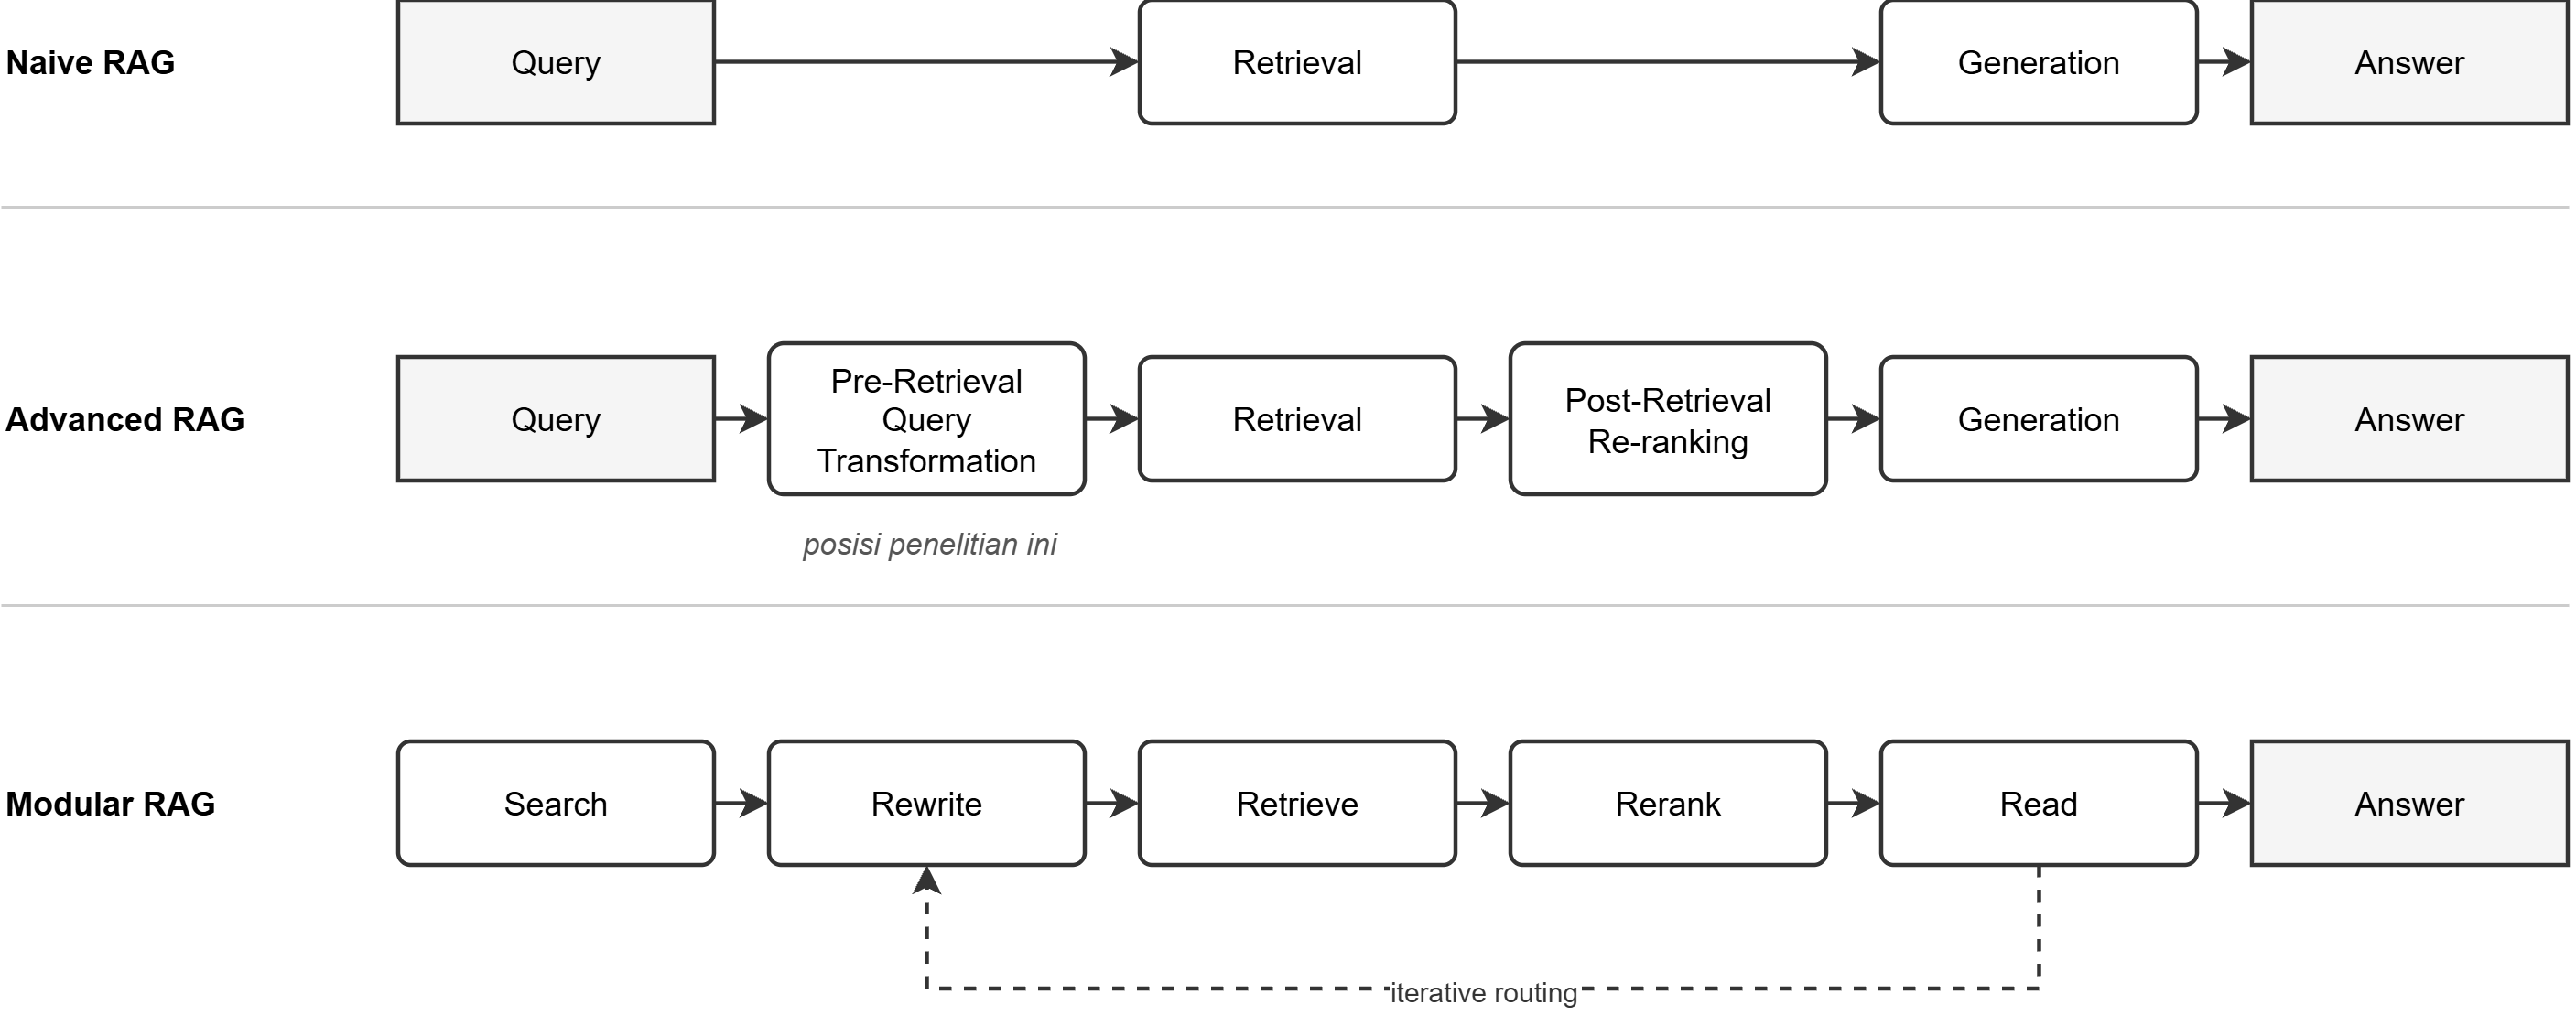
\includegraphics[width=\textwidth]{images/Gambar_II2_ParadigmaRAG.png}
\caption{Tiga paradigma RAG menurut \textcite{gao2023} beserta letak kontribusi penelitian ini.}
\label{fig:paradigma-rag}
\end{figure}

Gambar~\ref{fig:paradigma-rag} memperlihatkan bahwa kontribusi penelitian ini berada pada satu titik tertentu, yaitu tahap sebelum pencarian pada kelompok RAG canggih, sementara komponen lainnya mengikuti alur RAG standar. Penelitian ini menggunakan RAG standar sebagai tulang punggung, dengan dua penyesuaian dari kelompok RAG canggih. Penyesuaian pertama adalah penerapan \emph{Maximal Marginal Relevance} untuk menjaga keragaman dokumen yang diambil \autocite{carbonell1998}. Penyesuaian kedua, yang menjadi inti kontribusi penelitian ini, adalah transformasi kueri pada tahap sebelum pencarian. Penempatan ini penting untuk dinyatakan secara eksplisit agar tidak menimbulkan kesan bahwa penelitian ini mengusulkan arsitektur RAG yang sama sekali baru.

\subsection{Pengolahan Korpus dan Pemotongan Dokumen}
\label{subsec:pengolahan-korpus}

Sebelum penelusuran dapat dilakukan, dokumen sumber harus melewati tahap pengindeksan. Mutu tahap ini menentukan apakah konteks yang tepat dapat diperoleh pada tahap pencarian \autocite{gao2023}. Dokumen pedoman klinis umumnya berukuran puluhan hingga ratusan halaman, sehingga tidak dapat diperlakukan sebagai satu satuan penelusuran. Dokumen karena itu dipotong menjadi satuan yang lebih kecil, yang selanjutnya disebut potongan atau \emph{chunk}.

Penentuan ukuran potongan merupakan keputusan rancangan dengan konsekuensi yang saling bertolak belakang. \textcite{gao2023} menyatakan bahwa metode paling lazim adalah memotong dokumen berdasarkan jumlah token tetap, misalnya 100, 256, atau 512 token. Potongan yang besar memuat konteks lebih lengkap, tetapi turut membawa informasi yang tidak relevan sehingga menambah derau, memperpanjang waktu pemrosesan, dan meningkatkan biaya. Potongan yang kecil menghasilkan pencarian yang lebih tajam, tetapi berisiko memutus satu gagasan menjadi beberapa bagian sehingga tidak ada satu pun potongan yang memuatnya secara utuh. Risiko terakhir ini penting pada dokumen pedoman klinis, mengingat satu rekomendasi tata laksana kerap terdiri atas kondisi, tindakan, dan peringatan yang saling terkait. Ringkasan konsekuensi pemilihan ukuran potongan disajikan pada Tabel~\ref{tab:ukuran-potongan}.

\begin{table}[htbp]
\centering
\caption{Konsekuensi pemilihan ukuran potongan dokumen.}
\label{tab:ukuran-potongan}
\small
\begin{tabular}{@{}p{3.4cm}p{5.4cm}p{5.4cm}@{}}
\toprule
\textbf{Aspek} & \textbf{Potongan berukuran kecil} & \textbf{Potongan berukuran besar} \\
\midrule
Ketajaman pencarian & Lebih tajam karena setiap potongan memuat gagasan yang lebih sempit & Menurun karena satu potongan memuat beberapa gagasan sekaligus \\[2pt]
Keutuhan gagasan & Berisiko memutus satu rekomendasi menjadi beberapa bagian & Lebih terjaga karena kondisi, tindakan, dan peringatan cenderung berada dalam satu potongan \\[2pt]
Derau pada konteks & Rendah karena isi potongan lebih terfokus & Meningkat karena informasi yang tidak relevan turut terbawa \\[2pt]
Jumlah potongan & Banyak & Sedikit \\[2pt]
Biaya pemrosesan & Bertambah pada tahap pengindeksan seiring bertambahnya jumlah potongan & Bertambah pada tahap pembangkitan karena konteks yang dikirimkan lebih panjang \\
\bottomrule
\end{tabular}

\vspace{2pt}
\footnotesize Disarikan dari \textcite{gao2023}.\normalsize
\end{table}


Tabel~\ref{tab:ukuran-potongan} memperlihatkan bahwa tidak terdapat ukuran yang unggul pada seluruh aspek, sehingga penetapannya merupakan penyeimbangan antara ketajaman pencarian dan keutuhan makna, yang bergantung pada sifat dokumen yang diolah. Untuk mengurangi risiko pemutusan gagasan, potongan yang berdekatan dapat dibuat saling bertindih pada sebagian isinya. Dengan adanya pertindihan, kalimat yang berada tepat pada batas antara dua potongan tetap termuat secara utuh pada salah satunya. \textcite{gao2023} menyebut pendekatan ini sebagai salah satu teknik penyempurnaan pengindeksan, bersama dengan segmentasi yang lebih halus dan penyertaan metadata pada setiap potongan. Penyertaan metadata relevan bagi penelitian ini karena keterlacakan rekomendasi sampai ke nomor halaman dokumen sumber merupakan salah satu kebutuhan sistem, sebagaimana diuraikan pada Bab~\ref{chap:analisis-masalah}.

Setelah potongan dokumen diperoleh dan diubah menjadi representasi vektor, hasil pencarian tidak selalu langsung digunakan dalam urutan aslinya. Tahap pasca-penelusuran dapat menyertakan pemeringkatan ulang, yaitu menyusun kembali urutan potongan yang telah diperoleh agar isi yang paling relevan menempati posisi yang lebih diperhatikan oleh model bahasa \autocite{gao2023}. Kebutuhan akan tahap ini muncul karena model bahasa tidak memperlakukan seluruh bagian konteks secara setara, sebagaimana dibahas pada Subbab~\ref{subsec:rag-kesehatan}.

\subsection{Penerapan RAG pada Domain Kesehatan}
\label{subsec:rag-kesehatan}

Penerapan RAG pada domain kesehatan telah cukup mapan sehingga tidak perlu lagi dibuktikan dari awal dalam penelitian ini. Tinjauan sistematis oleh \textcite{amugongo2025} menelaah 70 studi terpilih dari 2.139 artikel pada periode 2020 sampai 2025 yang menerapkan RAG untuk membumikan model bahasa besar pada ranah medis. Tinjauan tersebut memetakan persoalan ke dalam tiga pertanyaan pokok, yaitu apa yang diambil, kapan pengambilan dilakukan, dan bagaimana hasil pengambilan digunakan.

Penelitian yang secara khusus membandingkan komponen RAG pada domain medis juga telah tersedia. \textcite{xiong2024} melakukan eksperimen berskala besar atas 41 kombinasi korpus, \emph{retriever}, dan model bahasa. Hasilnya menunjukkan bahwa penambahan komponen pencarian meningkatkan akurasi model bahasa hingga 18\% dibandingkan pendekatan tanpa pencarian. Penelitian tersebut juga menemukan efek \emph{lost-in-the-middle}, yaitu menurunnya kemampuan model memanfaatkan dokumen yang berada di tengah konteks ketika jumlah dokumen yang diambil terlalu banyak. Temuan ini menjadi dasar keputusan rancangan pada penelitian ini untuk membatasi jumlah dokumen yang diambil dan menerapkan pemeringkatan ulang, sehingga pemilihan konfigurasi tidak perlu dilakukan melalui pencarian eksploratif sendiri.

Pada tingkat penerapan, \textcite{kresevic2024} mengembangkan kerangka berbasis RAG untuk meningkatkan penafsiran pedoman klinis oleh model bahasa besar dalam konteks sistem pendukung keputusan dan melaporkan peningkatan akurasi dibandingkan model dasar. Kerangka tersebut menjadi acuan metodologis bagi penelitian ini karena kesamaan objek yang ditelusuri, yaitu dokumen pedoman klinis, serta kesamaan tujuannya, yaitu menghasilkan rekomendasi yang dibumikan pada pedoman.

Penerapan RAG pada ranah diabetes secara khusus juga telah dilaporkan. \textcite{lee2024} membangun sistem RAG ganda yang dibumikan pada pedoman diabetes terkini dan melaporkan berkurangnya halusinasi pada keluaran model bahasa. \textcite{wang2024} menerapkan RAG untuk edukasi diabetes dan melaporkan peningkatan pada akurasi, kelengkapan, serta keterpahaman jawaban. Kedua penelitian tersebut memperlihatkan bahwa pedoman diabetes merupakan objek penelusuran yang layak bagi RAG, sekaligus memperlihatkan pola yang seragam pada penelitian terdahulu. Kueri penelusuran pada keduanya berasal dari pertanyaan pengguna atau dari kondisi yang sedang berlaku, sehingga panduan yang diperoleh menanggapi keadaan yang telah teramati.

Pada sisi yang berbeda, penelitian yang mempertemukan model bahasa besar dengan peramalan kadar glukosa menempuh arah yang terpisah dari arah tersebut. Penelitian pada arah ini menempatkan model bahasa sebagai pelaku peramalan itu sendiri, yaitu memanfaatkan kemampuannya memodelkan deret untuk menghasilkan taksiran kadar glukosa, dan bukan sebagai penyusun rekomendasi yang dikondisikan pada keluaran suatu prediktor. Dengan demikian, kedua arah tersebut berkembang tanpa saling bertaut. Penelusuran panduan klinis belum dikondisikan pada keluaran prediktor mengenai kondisi pasien pada waktu yang akan datang.

\subsection{Transformasi Kueri dan Pengondisian pada Prediksi}
\label{subsec:transformasi-kueri}

Transformasi kueri merupakan teknik baku pada tahap sebelum pencarian, ketika kueri yang dikirimkan ke \emph{retriever} bukan merupakan masukan mentah melainkan hasil pengolahan terlebih dahulu \autocite{gao2023}. Penelitian ini menerapkan teknik tersebut dengan strategi khusus, yaitu kueri dibangun dari kadar glukosa yang diprediksi untuk 30 sampai 60 menit ke depan, bukan dari kondisi pasien saat ini. Strategi ini selanjutnya disebut \emph{query transformation} terkondisi-prediksi. Alur RAG konvensional yang menjadi titik tolak ditunjukkan pada Gambar~\ref{fig:rag-konvensional}.

\begin{figure}[htbp]
\centering
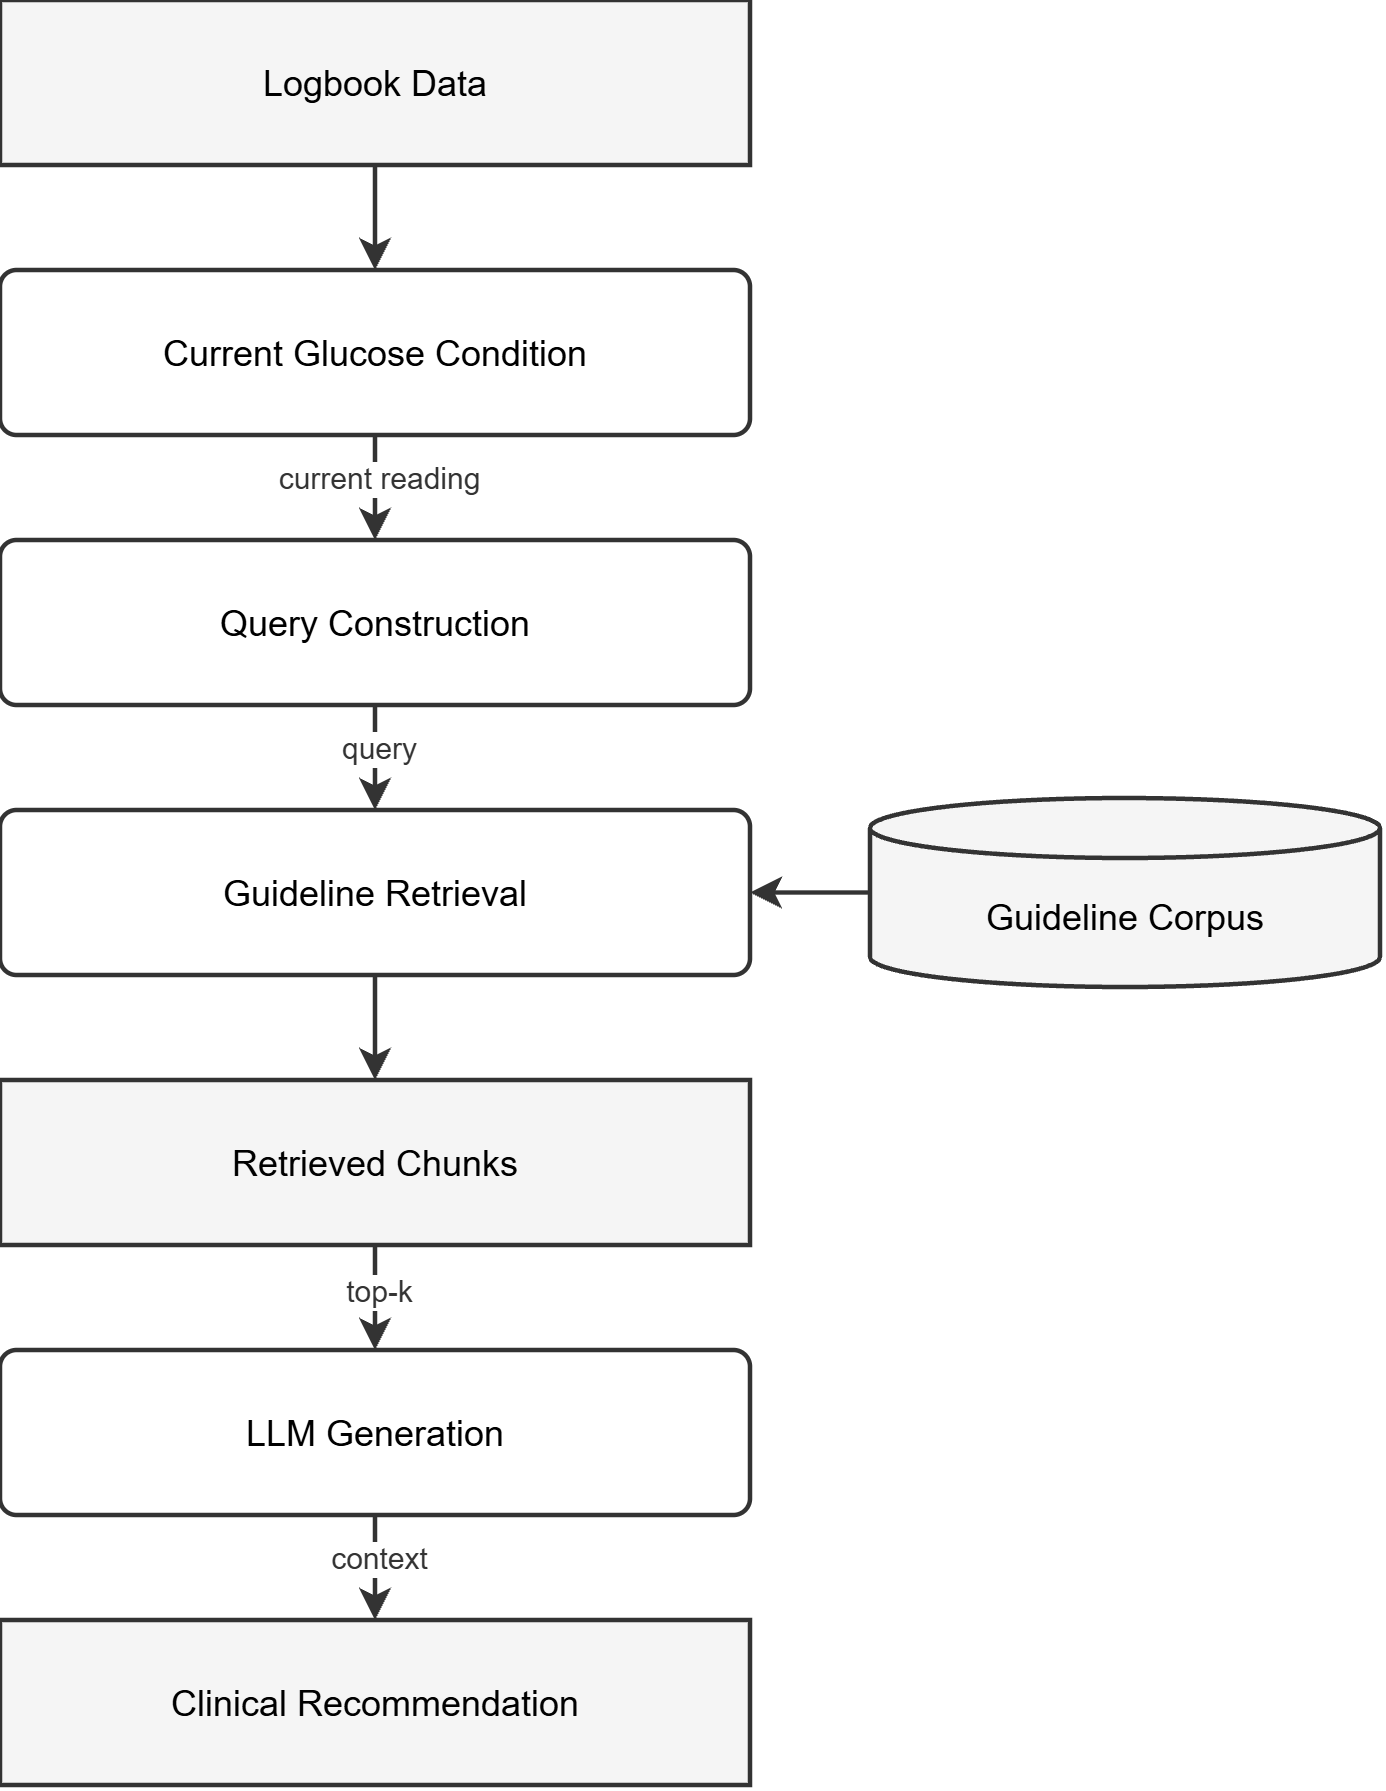
\includegraphics[width=0.62\textwidth]{images/Gambar_II3_AlurRAGKonvensional.png}
\caption{Alur RAG konvensional, dengan kueri yang dibangun dari kondisi glukosa yang sedang berlaku.}
\label{fig:rag-konvensional}
\end{figure}

Gambar~\ref{fig:rag-konvensional} memperlihatkan bahwa data \emph{logbook} langsung diterjemahkan menjadi kondisi glukosa saat ini, sehingga kondisi itulah yang menyusun kueri penelusuran. Panduan yang diperoleh karena itu menanggapi keadaan yang telah teramati. Alur yang diusulkan penelitian ini ditunjukkan pada Gambar~\ref{fig:rag-terkondisi}.

\begin{figure}[htbp]
\centering
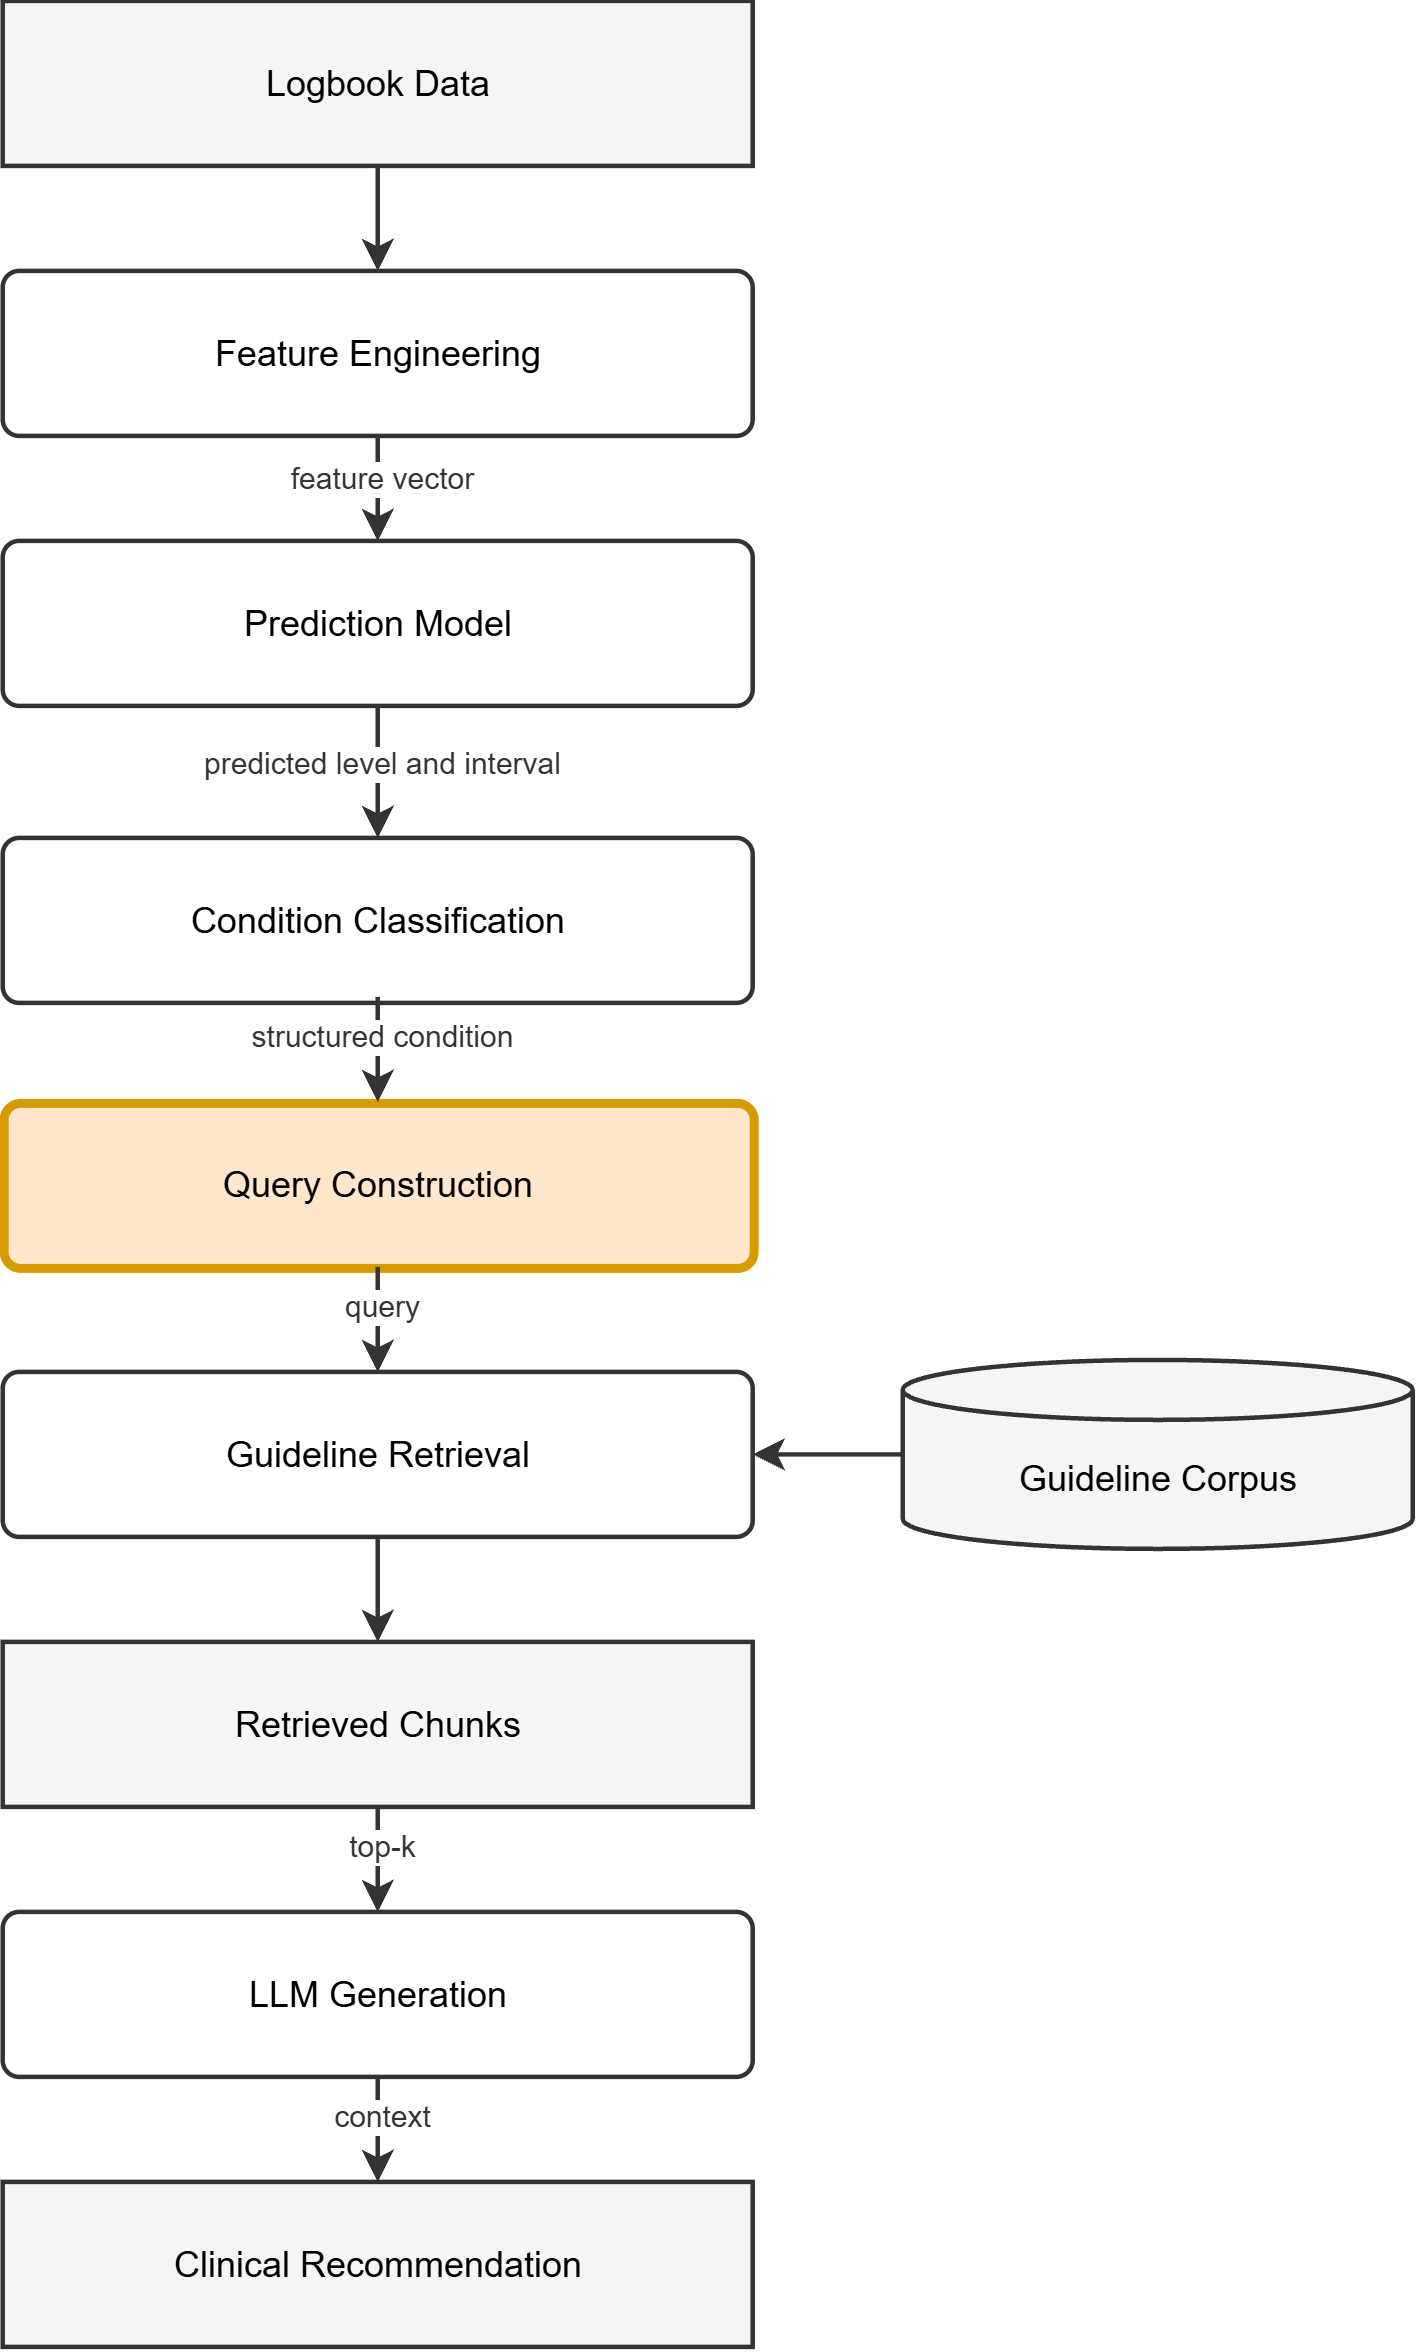
\includegraphics[width=0.62\textwidth]{images/Gambar_II4_AlurRAGTerkondisiPrediksi.png}
\caption{Alur RAG terkondisi-prediksi. Kotak bergaris tebal menandai tahap yang membedakannya terhadap Gambar~\ref{fig:rag-konvensional}.}
\label{fig:rag-terkondisi}
\end{figure}

Gambar~\ref{fig:rag-terkondisi} memperlihatkan bahwa tiga tahap disisipkan sebelum penyusunan kueri, yaitu rekayasa fitur, model prediksi, dan klasifikasi kondisi. Perlu ditegaskan bahwa modul \emph{machine learning} pada penelitian ini tidak ditempatkan setelah RAG, melainkan mendahului dan mengondisikannya. Keluaran prediksi digunakan untuk membentuk kueri, sehingga dokumen yang diambil dan rekomendasi yang dihasilkan mengacu pada kondisi yang akan datang. Perbedaannya dengan alur konvensional terletak pada asal-usul kueri, bukan pada mekanisme pencarian maupun pembangkitannya.

Terdapat beberapa pendekatan lain yang secara sekilas tampak serupa sehingga perlu dibedakan secara eksplisit. Pendekatan \emph{forward-looking active retrieval} \autocite{jiang2023} juga bersifat antisipatif, tetapi pengondisiannya bersumber dari prediksi model bahasa atas kalimat yang akan ia tulis sendiri, bukan dari prediktor eksternal atas kondisi fisiologis pasien. Pendekatan lain mengondisikan pencarian pada keadaan sistem yang sedang berlangsung, sehingga tetap mengacu pada kondisi saat ini. Dengan demikian, sejauh penelusuran yang dilakukan pada Subbab~\ref{subsec:rag-kesehatan} dan Subbab~\ref{sec:penelitian-terkait}, pengondisian pencarian panduan klinis pada keluaran prediktor eksternal mengenai kondisi pasien pada waktu yang akan datang belum dijumpai pada literatur terdahulu.

\subsection{Evaluasi Sistem Penelusuran dan Pembangkitan}
\label{subsec:evaluasi-rag}

Penilaian sistem RAG mencakup dua sisi yang berbeda, yaitu mutu penelusuran dan mutu jawaban yang dibangkitkan. Kedua sisi tersebut diukur dengan kelompok metrik yang berlainan.

Mutu penelusuran dinilai menggunakan metrik yang lazim pada bidang pencarian informasi. Metrik tersebut tidak hanya memperhatikan apakah dokumen yang relevan berhasil diperoleh, melainkan juga pada peringkat keberapa dokumen tersebut muncul, karena pengguna maupun model bahasa memberi perhatian lebih besar pada hasil di posisi awal \autocite{manning2008}. Dua metrik yang digunakan pada penelitian ini adalah Hit@k dan \emph{mean reciprocal rank}. Hit@k menyatakan proporsi kueri yang memperoleh dokumen relevan di antara $k$ hasil teratas, sehingga menunjukkan apakah dokumen yang dibutuhkan berhasil dijangkau. \emph{Mean reciprocal rank} menyatakan rata-rata dari kebalikan peringkat dokumen relevan pertama, sehingga memberi nilai lebih tinggi ketika dokumen relevan muncul lebih awal \autocite{manning2008}.

Mutu jawaban yang dibangkitkan dinilai menggunakan kerangka evaluasi seperti RAGAS \autocite{es2023}, yang mengukur aspek seperti kesetiaan jawaban terhadap konteks yang diperoleh dan relevansi jawaban terhadap pertanyaan. Kerangka tersebut menilai keluaran akhir sistem, sehingga bersifat melengkapi metrik penelusuran yang hanya menilai tahap pencarian. Ringkasan kedua kelompok metrik tersebut disajikan pada Tabel~\ref{tab:metrik-evaluasi}.

\begin{table}[htbp]
\centering
\caption{Metrik evaluasi sistem penelusuran dan pembangkitan.}
\label{tab:metrik-evaluasi}
\small
\begin{tabular}{@{}p{3.0cm}p{5.5cm}p{1.8cm}p{2.3cm}@{}}
\toprule
\textbf{Metrik} & \textbf{Aspek yang diukur} & \textbf{Rentang} & \textbf{Rujukan} \\
\midrule
\multicolumn{4}{@{}l}{\emph{Mutu penelusuran}} \\[2pt]
Hit@k & Apakah potongan relevan terjangkau di antara $k$ hasil teratas & 0 sampai 1 & \textcite{manning2008} \\[2pt]
\emph{Mean reciprocal rank} & Seberapa awal potongan relevan pertama muncul pada daftar hasil & 0 sampai 1 & \textcite{manning2008} \\[4pt]

\multicolumn{4}{@{}l}{\emph{Mutu pembangkitan}} \\[2pt]
\emph{Faithfulness} & Kesetiaan jawaban terhadap konteks yang diperoleh & 0 sampai 1 & \textcite{es2023} \\[2pt]
\emph{Answer relevancy} & Relevansi jawaban terhadap pertanyaan yang diajukan & 0 sampai 1 & \textcite{es2023} \\[2pt]
\emph{Context precision} & Proporsi konteks yang diambil yang benar-benar relevan & 0 sampai 1 & \textcite{es2023} \\[2pt]
\emph{Context recall} & Proporsi konteks relevan yang berhasil diambil & 0 sampai 1 & \textcite{es2023} \\[4pt]

\multicolumn{4}{@{}l}{\emph{Mutu dan keamanan prediksi}} \\[2pt]
RMSE dan MAE & Besar galat prediksi terhadap nilai aktual & mg/dL & --- \\[2pt]
\emph{Clarke Error Grid} & Konsekuensi klinis dari galat, dipetakan ke zona A sampai E & zona A--E & \textcite{clarke1987} \\[2pt]
Sensitivitas dan PPV & Kemampuan mengenali kejadian hipoglikemia dan keandalan peringatannya & 0 sampai 1 & --- \\[2pt]
Cakupan konformal & Proporsi nilai aktual yang tercakup interval prediksi & 0 sampai 1 & \textcite{angelopoulos2021} \\
\bottomrule
\end{tabular}

\vspace{2pt}
\footnotesize Rumusan matematis setiap metrik disajikan pada Bab~\ref{chap:evaluasi} agar dapat disertai penjelasan komponennya.\normalsize
\end{table}


Tabel~\ref{tab:metrik-evaluasi} memperlihatkan bahwa metrik penelusuran dan metrik pembangkitan saling melengkapi. Hit@k menjawab pertanyaan apakah dokumen relevan terjangkau, sedangkan \emph{mean reciprocal rank} menjawab pertanyaan seberapa awal dokumen tersebut muncul. Nilai $k$ yang terlalu besar dapat membuat Hit@k menjadi jenuh pada korpus berukuran kecil, sehingga kemampuannya membedakan antarsistem berkurang dan penilaian bertumpu pada metrik peringkat. Rumusan matematis setiap metrik tidak disajikan pada tabel ini, melainkan pada Bab~\ref{chap:evaluasi}, agar setiap persamaan dapat disertai penjelasan komponennya.

\section{Penelitian Terkait dan Posisi Penelitian}
\label{sec:penelitian-terkait}

Penelitian terdahulu yang relevan dapat dikelompokkan ke dalam tiga arah. Arah pertama berfokus pada prediksi glukosa berbasis data tanpa menghasilkan rekomendasi dalam bahasa alami. Arah kedua berfokus pada pengelolaan diabetes berbasis representasi pengetahuan terstruktur yang menuntut infrastruktur besar. Arah ketiga berfokus pada penerapan RAG untuk penafsiran pedoman klinis, tetapi dengan kueri yang dibangun dari kondisi yang sedang berlaku.

\textcite{woldaregay2019} menegaskan kelayakan pemodelan berbasis data untuk memprediksi dinamika glukosa pada DMT1, namun keluarannya berhenti pada nilai prediksi tanpa disertai panduan tindakan. \textcite{ghimire2024} menguji kemampuan generalisasi model \emph{deep learning} antar-dataset dan menemukan bahwa kinerjanya menurun ketika diterapkan pada data yang berbeda dari data pelatihan. \textcite{rad2024} mengembangkan kerangka pengelolaan diabetes berbasis \emph{personal health knowledge graph} dengan penelusuran SPARQL, yang mampu menghasilkan berbagai layanan personal tetapi mensyaratkan ontologi formal, integrasi rekam medis, dan pemantauan kontinu. \textcite{kresevic2024} menunjukkan bahwa RAG meningkatkan mutu penafsiran pedoman klinis, dengan kueri yang dibangun dari kondisi yang sedang berlaku. Pada ranah diabetes secara khusus, \textcite{lee2024} dan \textcite{wang2024} memperlihatkan bahwa pembumian pada pedoman diabetes menekan halusinasi sekaligus meningkatkan mutu jawaban, dengan kueri yang bersumber dari pertanyaan pengguna. Ringkasan penelitian terkait beserta posisi penelitian ini disajikan pada Tabel~\ref{tab:penelitian-terkait}.

\begin{longtable}{@{}p{2.6cm}p{3.1cm}p{2.5cm}p{3.0cm}p{3.0cm}@{}}
\caption{Ringkasan penelitian terkait dan posisi penelitian ini.}
\label{tab:penelitian-terkait} \\
\toprule
\textbf{Peneliti} & \textbf{Fokus atau pendekatan} & \textbf{Jenis data} & \textbf{Temuan} & \textbf{Keterbatasan} \\
\midrule
\endfirsthead

\multicolumn{5}{@{}l}{\small\emph{Tabel \thetable{} (lanjutan)}} \\
\toprule
\textbf{Peneliti} & \textbf{Fokus atau pendekatan} & \textbf{Jenis data} & \textbf{Temuan} & \textbf{Keterbatasan} \\
\midrule
\endhead

\bottomrule
\endlastfoot

\textcite{woldaregay2019} & Tinjauan pemodelan berbasis data untuk prediksi dinamika glukosa pada DMT1 & Pemantauan kontinu dan data multimoda & Pemodelan berbasis data layak untuk memprediksi dinamika glukosa & Keluaran berhenti pada nilai prediksi tanpa panduan tindakan \\[2pt]

\textcite{ghimire2024} & Pengujian generalisasi model \emph{deep learning} antar-dataset & Beberapa dataset pemantauan kontinu & Kinerja menurun ketika diterapkan pada data yang berbeda dari data pelatihan & Tidak menghasilkan rekomendasi dalam bahasa alami \\[2pt]

\textcite{rad2024} & Pengelolaan diabetes berbasis \emph{personal health knowledge graph} dengan penelusuran SPARQL & Rekam medis terintegrasi dan pemantauan kontinu & Mampu menghasilkan berbagai layanan personal di atas graf pengetahuan & Menuntut ontologi formal, integrasi rekam medis, dan pemantauan kontinu. Penelusuran ditujukan pada data pasien, bukan pada dokumen pedoman \\[2pt]

\textcite{kresevic2024} & RAG untuk meningkatkan penafsiran pedoman klinis pada sistem pendukung keputusan & Dokumen pedoman klinis & Penelusuran pedoman meningkatkan akurasi dibandingkan model dasar & Kueri dibangun dari kondisi yang sedang berlaku \\[2pt]

\textcite{lee2024} & Sistem RAG ganda yang dibumikan pada pedoman diabetes & Dokumen pedoman diabetes & Halusinasi pada keluaran model bahasa berkurang & Kueri bersumber dari pertanyaan pengguna \\[2pt]

\textcite{wang2024} & RAG untuk edukasi diabetes & Dokumen pedoman diabetes & Akurasi, kelengkapan, dan keterpahaman jawaban meningkat & Kueri bersumber dari pertanyaan pengguna \\[2pt]

\textcite{jiang2023} & Penelusuran aktif yang bersifat antisipatif & Dokumen umum & Penelusuran dipicu ketika model bahasa kurang yakin atas kalimat yang akan ditulisnya & Pengondisian bersumber dari prediksi model bahasa atas teksnya sendiri, bukan dari prediktor eksternal \\[2pt]

\textbf{Penelitian ini} & CDSS yang memadukan modul prediksi glukosa dengan RAG pedoman klinis melalui \emph{query transformation} terkondisi-prediksi & Data \emph{logbook} periodik dan korpus dua belas dokumen pedoman & Kueri penelusuran dibangun dari kadar glukosa terprediksi, sehingga panduan yang diperoleh bersifat antisipatif & Bersifat \emph{proof-of-concept} tanpa uji klinis, dan mutu penelusuran bergantung pada cakupan korpus \\

\end{longtable}


Tabel~\ref{tab:penelitian-terkait} memperlihatkan satu pola yang berulang pada seluruh penelitian terdahulu tersebut. Penelitian pada arah pertama menghasilkan taksiran mengenai kondisi yang akan datang tetapi berhenti pada nilai prediksi, sedangkan penelitian pada arah kedua dan ketiga menghasilkan rekomendasi dalam bahasa alami tetapi menyusun kuerinya dari kondisi yang sedang berlaku atau dari pertanyaan pengguna. Kedua kelompok tersebut berkembang tanpa saling bertaut, sehingga taksiran mengenai kondisi yang akan datang belum pernah dijadikan dasar penelusuran panduan klinis.

Posisi penelitian ini berada pada perpotongan ketiga arah tersebut. Penelitian ini mengadopsi kerangka RAG berbasis pedoman klinis sebagaimana \textcite{kresevic2024}, menggunakan modul prediksi berbasis data sebagaimana arah pertama, kemudian menghubungkan keduanya melalui pengondisian kueri pada keluaran prediksi. Hubungan inilah yang membedakannya dari penelitian terdahulu, karena pada penelitian sebelumnya modul prediksi dan modul rekomendasi berjalan terpisah tanpa saling mengondisikan. Adapun \textcite{rad2024} dipertahankan pada pembahasan ini bukan sebagai kerangka yang diperluas, melainkan sebagai pembanding yang menunjukkan batas keterterapan pendekatan berbasis representasi pengetahuan terstruktur pada lingkungan dengan sumber daya terbatas.
